\section{Ergebnis} % (fold)
\label{sec:ergebnis}
	\subsubsection{Wie wurde getestet?} % (fold)
	\label{ssub:wie_wurde_getestet}
	
	% subsubsection wie_wurde_getestet (end)
		Bereits zu Beginn des Projekts war es wichtig es messbar zu machen. Dafür wurde eine Testumgebung aufgebaut, mit deren Hilfe die Seite nach ihrer Geschwindigkeit getestet werden kann. Ganz entscheidend war dabei die Webpagetest API in Verbindung mit Google Spreadsheets. Damit ließen sich die Tests regelmäßig automatisiert ausführen und die Daten wurden automatisch in einer Tabelle gespeichert. Die volle Sammlung der Daten über den Zeitraum der Arbeit hinweig ist hier zu finden: \url{http://tinyurl.com/l5usz79}. Diese Daten wurden in Diagrammen aufbereitet und sind unter: \url{http://bithugger.github.io/bachelorthesis/} zu finden.

		1089 Testläufe über Webpagtest: Zeitraum: 1 Monat

		\begin{figure}[htbp]
			\begin{center}
				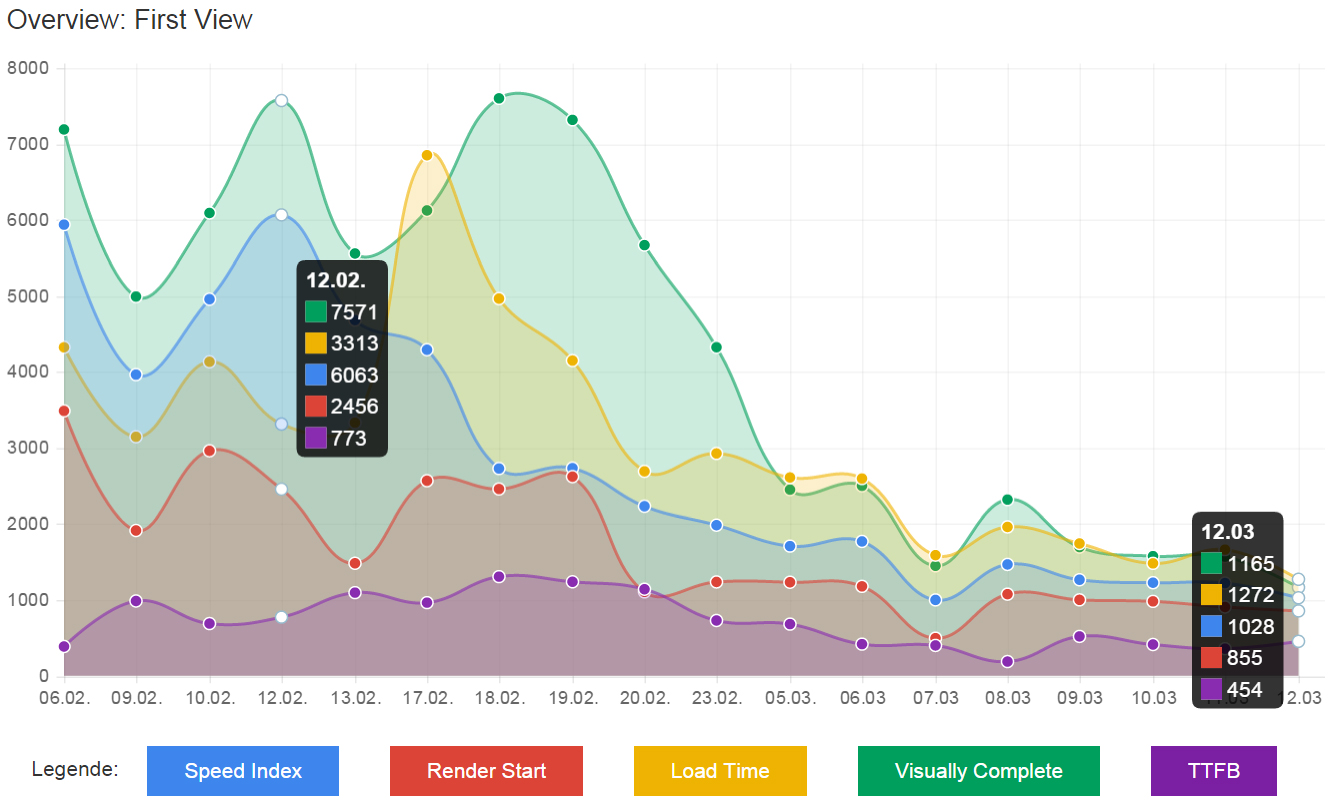
\includegraphics[width=\textwidth]{data_all.jpg}
				\caption{...}
				\label{fig:data_all}
			\end{center}
		\end{figure}
		
		todo

	% section ergebnis (end)
